
Since plane cuts an intercept of 3 units on y-axis, point $\vec{C}=\myvec{0\\3\\0}$ lies on the plane.\\
Also, as the plane is parallel to the ZOX plane, both must have same normal vector. So,
\begin{align}
    \vec{n}=\vec{n}_{\text{ZOX}}=\myvec{0\\1\\0}
\end{align}
If $\vec{x}$ is a general point on the plane, then the equation of plane is given by
\begin{align}
    &\vec{n}^\top(\vec{x}-\vec{C})=0\\
    \implies &\vec{n}^\top\vec{x}=\vec{n}^\top\vec{C}\\
    \implies &\myvec{0&1&0}\vec{x}=\myvec{0&1&0}\myvec{0\\3\\0}\\
    \implies &\myvec{0&1&0}\vec{x}=3
\end{align}
See Fig.          \ref{aug/2/26/plot} for a verification.
\begin{figure}[!ht]
\centering
         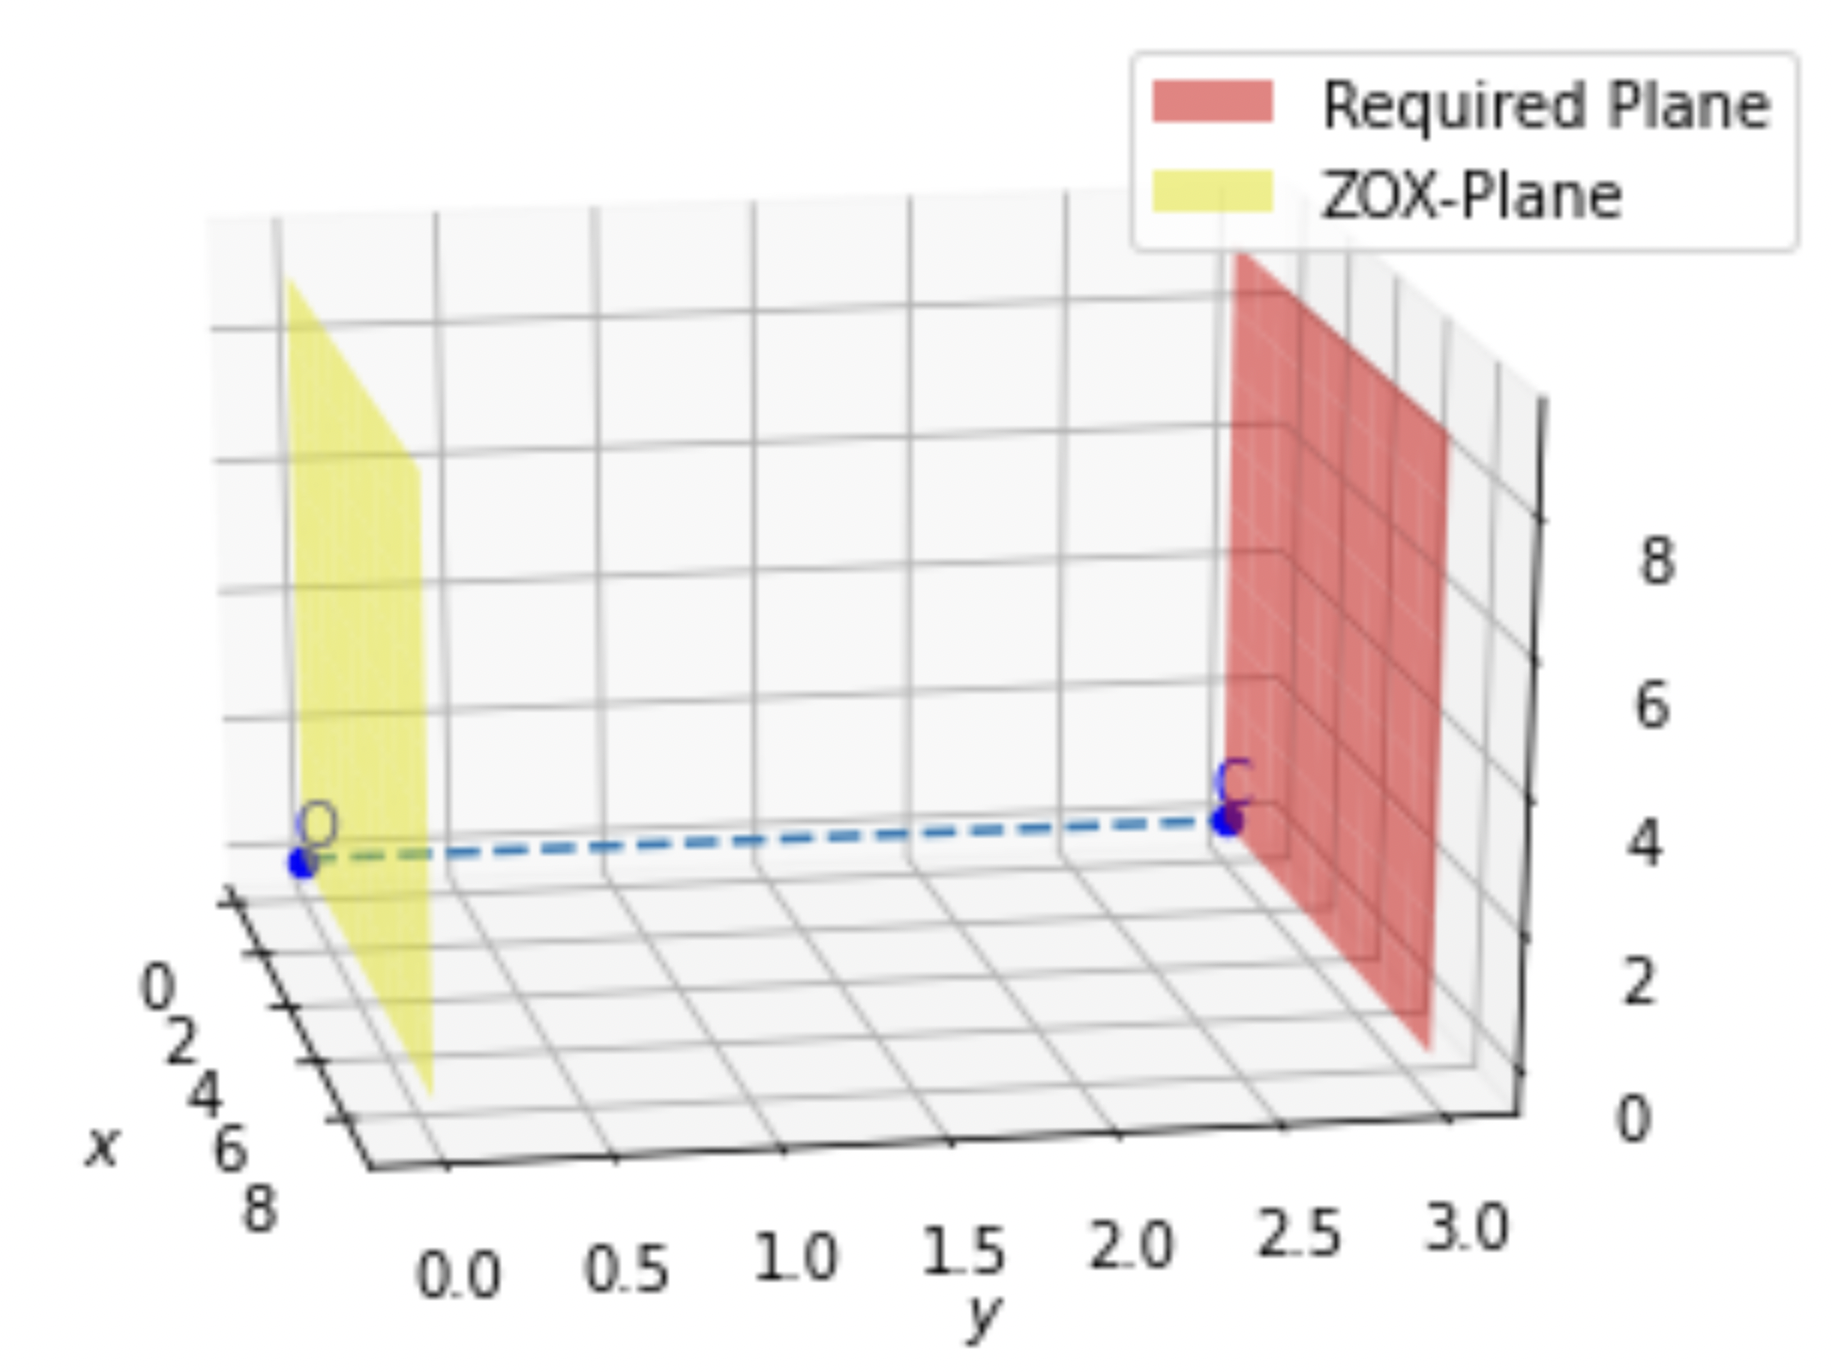
\includegraphics[width=\columnwidth]{solutions/aug/2/26/figures/figure.png}
         \caption{3D plot}
         \label{aug/2/26/plot}
\end{figure}

